\section{Formati immagine}
Il formato è la regola con la quale una descrizione dell'immagine è memorizzata in un file elettronico, che comprende sia i dati che le modalità di lettura e interpretazione.

\subsection{Bitmap}
Bitmap è il formato più indicato per le immagini a \textbf{3 canali di 8 bit}, ma supporta anche profondità differenti. Il numero di bit necessari dipende dal numero di pixel, applicando un fattore moltiplicativo di 24.

A livelli di grigio utilizza i tre colori uguali, memorizzando le immagini dal basso a sinistra riga per riga, con header e mappa di colori.

La compressione non introduce perdita, utilizzando RLE: questo metodo può eventualmente fallire in caso di pattern disomogenei. 

\subsection{GIF}
GIF (Graphics Interchange Format) permette la sovrapposizione tra immagini, attivando la \textbf{trasparenza uniforme} 0-1. Può contenere più immagini, quindi può essere utilizzato per le animazioni.

Si usa quando l'immagine originale è a scala di colore, con un massimo di 256 colori. La compressione è senza perdita, ma la limitazione di 256 colori (8 bit) quantizza pesantemente il numero di combinazioni a disposizione.

\subsection{TIFF}
TIFF (Tagged Image File Format) gestisce immagini con contenuti ad altissime frequenze, sfruttando algoritmi che cercano \textbf{ripetizioni di pattern} (loghi) a discapito delle dimensioni.

Permette di salvare caratteristiche aggiuntive memorizzando le informazioni colore in spazi diversi, definendo profili standard per allineare risposte di devices differenti.

Può essere salvato con o senza compressione, in caso adottando conservazione come LZW.

TIFF contiene meta informazioni in locazioni di memoria chiamate tag, che includono per esempio risoluzione, compressione o modello di colore.

 \subsection{PNG}
 PNG (Portable Network Graphics) è una valida alternativa a GIF con diverse profondità colore, fino a 48 bit. Un ulteriore passaggio è l'\textbf{alpha-channel} per gestire la trasparenza, estendendo 0-1 a più livelli. 
 
 PNG è utile per lo scambio di informazioni su internet, senza la limitazione colore. La compressione è lossless con dimensioni inferiori rispetto a TIFF, utilizzando un alpha channel per la trasparenza.
 
 L'alpha-channel assume valori tra 0 e 1, e indica le modalità di blending tra più immagini, secondo la formula:
 $$\alpha I_A + (1 - \alpha) I_B$$
 
 \subsection{JPEG}
 JPEG (Joint Photographic Experts Group) memorizza \textbf{immagini fotografiche} con perdita di informazioni, tramite RGB, CMYK o scale di grigio.
 
 Non supporta la trasparenza e tratta solo immagini statiche, mentre per i filmati viene usato MPEG. Come formato intermedio per una sequenza di passi di manipolazione non è indicato, mentre TIFF è ottimale.
 
 \subsubsection{JPEG-2000}
 JPEG-2000 è basato su tecnologie \textbf{wavelet} per una migliore compressione, senza artefatti a blocchi. Ha il supporto per multi-spectral imagery e la capacità di ricostruzione progressiva dell'immagine codificando regioni di interesse.
 
 \begin{figure}[h]
 	\centering
 	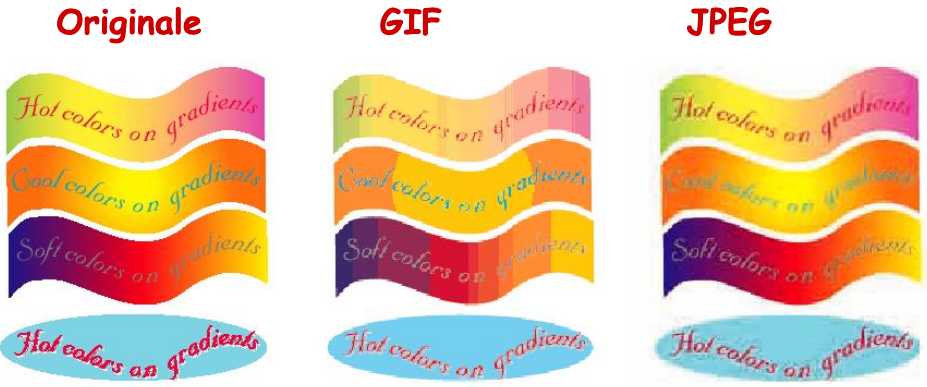
\includegraphics[scale=0.4]{Lezioni/Immagini/formati}
 \end{figure}
 
 \subsection{Postscript}
 Postscript è basato su una descrizione \textbf{vettoriale}, definendo gli elementi di pagina come vettori. Immagini bitmap possono essere inclusi nei file, insieme a informazioni addizionali memorizzate senza compressione (ASCII).
 
 \subsection{PDF}
 PDF (Portable Document Format) consiste in una o più \textbf{pagine} che conservano font, formattazione e colori del sorgente. Può contenere grafica vettoriale, immagini, video e link a ipertesti.
 
 Supporta la compressione JPEG, RLE e LZW, con profili ICC.
 
 \subsection{SVG}
 SVG è un linguaggio per la grafica 2D che sostituisce Postscript, per visualizzare sul web \textbf{immagini vettoriali}, bitmap e testo.
 
 \subsection{EXIF}
 EXIF è un formato per immagini da \textbf{camera digitale}. Contiene numerosi tag, come TIFF, con informazioni sulla camera e sulle condizioni di acquisizione. Lo standard EXIF include anche specifiche per l'audio.
 
 I tag si suddividono in:
 \begin{itemize}
 	\item Tag che riguardano la fotocamera;
 	\item Tag che riguardano l'immagine;
 	\item Altri tag.
 \end{itemize}
 
 \section{Compressione audio}
 La compressione audio è legata a strategie predittive tramite \textit{interpolazione dei valori} o modelli basati su come alcuni suoni possono apparire (es. parlato), senza introdurre perdita e con rapporti di compressione dipendenti dal tipo di audio: il silenzio può essere eliminato, e i suoni artificiali vengono predetti più difficilmente.
 
 I fattori da considerare sono:
 \begin{itemize}
 	\item Riduzione dei livelli di quantizzazione, con un alto rapporto di compressione e un deterioramento di SNR;
 	\item Riduzione della frequenza di campionamento, con perdita delle informazioni ad alta frequenta e aliasing.
 \end{itemize}

Oltre alla compressione del silenzio, si può adattare DCPM con codifica entropica lossless.

Gli algoritmi lossy basati su predizione includono:
\begin{itemize}
	\item ADCPM, che predice il valore di un campione a partire dal valore di più campioni precedenti, e codifica l'errore quantizzando;
	\item LCP e CELP per il parlato, che sfruttano un modello vocale e ne trasmettono i parametri.
\end{itemize}

Un altro aspetto da sfruttare riguarda gli altri meccanismi dei sistemi umani: il mascheramento e la non linearità degli effetti. 
 
Un modo più efficace tiene conto del \textbf{sistema percettivo}, eliminando le frequenze fuori dal range di udibilità applicando un filtro passa-banda e rimuovendo gli alias. 

Le curve isofone rapresentano i suoni percepiti con lo stesso volume (pressione acustica o intensità sonora), in foni. Il volume percepito dipende dall'intensità e dalla frequenza, e ha come diretta conseguenza il mascheramento in frequenza, cioè l'innalzamento della soglia di udibilità.

\begin{figure}[h]
	\centering
	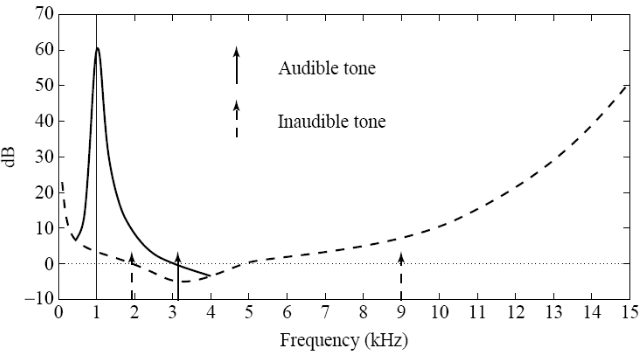
\includegraphics[scale=0.6]{Lezioni/Immagini/mascheramento}
\end{figure}
 
Il suono \textbf{mascherante} è il suono disturbatore, mentre il suono \textbf{mascherato} è il suono mascherato. Quest'ultimo è condizionato dalla diminuzione di sensibilità, e il mascheramento si misura con l'aumento di intensità necessario per tornare udibile.
 
Maggiore è la frequenza del tono che maschera, maggiore è il suo effetto, cioè è più ampia la banda di frequenze che maschera.
 
L'udito umano ha una risoluzione limitata in funzione della frequenza, comportandosi come un filtro passa-banda senza principio di sovrapposizione degli effetti.
 
La \textbf{banda critica} è un intervallo di frequenze in cui \textit{le frequenze vengono mescolate}, e due toni puri simultanei non possono essere percepiti come distinti. Se la distanza è superiore alla banda critica, la sensazione sonora è doppia (pari alla somma delle sensazioni simili); altrimenti, è inferiore.

Per ogni range di frequenze udibili, esiste una banda critica larga costante fino a 500 Hz, che poi aumenta linearmente con la frequenza. L'effetto di mascheramento è maggiore se l'intervallo tra frequenza mascherante e mascherata è contenuto in una banda critica.

Ogni suono ad alta intensità provoca una saturazione dei recettori all'interno dell'orecchio, che richiedono del tempo per poter ripristinare le condizione iniziale. Più è lunga la durata del suono mascherante, maggiore è il tempo.

Mascheramento \textbf{in frequenza}:
\begin{enumerate}
	\item Un tono più basso può mascherare un tono più alto e viceversa;
	\item Maggiore è la potenza/frequenza del tono che maschera, più è ampia la banda di frequenze che maschera.
\end{enumerate}

Mascheramento \textbf{temporale}:
\begin{enumerate}
	\item Maggiore è la potenza/durata del tono che maschera, maggiore è il tempo necessario per ripristinare l'udibilità;
	\item Minore è la potenza del tono mascherato, maggiore è il tempo necessario per udirlo.
\end{enumerate}

L'obiettivo è la rimozione delle parti di un segnale audio acusticamente irrilevanti, in modo da non percepire il rumore di quantizzazione.

 \subsection{MPEG}
MPEG coding algorithm: il tono mascherato viene modificato una volta individuata la banda con il tono più alto, osservando la potenza nelle bande vicine. Considerato un frame, si trova il tono mascherante, e in base a esso si osserva come viene modificata la soglia di udibilità in modo da poter eliminare i suoni non percepiti. 

\begin{figure}[h]
	\centering
	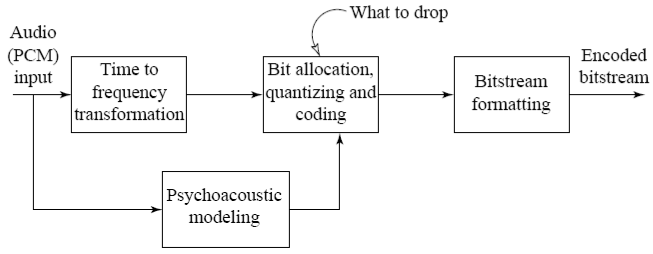
\includegraphics[scale=0.5]{Lezioni/Immagini/mpeg-coding-audio}
\end{figure}

Le frequenze sono scomposte, e il segnale audio è codificato con una rappresentazione spettrale. L'output dei filtri è poi quantizzato eliminando il rumore nella soglia di mascheramento, e vengono trasmesse le componenti in frequenza che sono state mascherate con un numero minore di bit.

MPEG applica 32 bande che simulano le bande critiche. A bassa frequenza esse si sovrappongono, e la banda con effetto minimo vincola i bit per l'intera banda. Ad alta frequenza, invece, una banda critica corrisponde a diverse bande, a discapito della potenza di calcolo.

La codifica è composta da tre strati (Sub Band Coder) indipendenti, che sfruttano progressivamente la complessità del modello psicoacustico e la compressione: 
\begin{enumerate}
	\item Algoritmo di qualità abbastanza buona;
	\item Maggiore compressione con maggiore costo di encoder e decoder;
	\item Adaptive Transform Coding, con maggiore complessità in codifica.
\end{enumerate}

\begin{figure}[h]
	\centering
	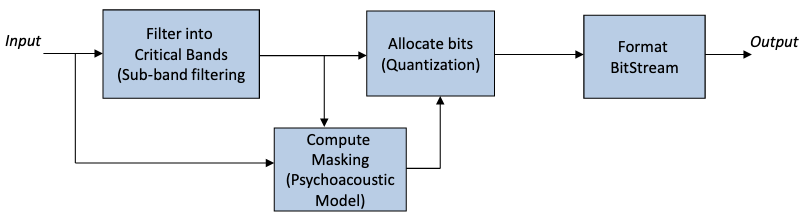
\includegraphics[scale=0.5]{Lezioni/Immagini/mpeg-coding}
\end{figure}

\begin{enumerate}
	\item Il segnale audio è convertito e diviso (componenti spettrali) in 32 sottobande di frequenza;
	\item Per ciascuna sottobanda, il mascheramento è applicato in base al modello psicoacustico scelto;
	\item Se la potenza in una banda, calcolata con una spreading function, è inferiore alla soglia di mascheramento, la banda mascherata non viene codificata;
	\item Altrimenti, vengono determinati i bit necessari a rappresentare il coefficiente in modo da mascherare il rumore di quantizzazione;
	\item I componenti che superano la soglia vengono codificati con Huffman.
\end{enumerate}

La soglia di udibilità viene calcolata in base alla minima soglia di mascheramento o in base alla media di esse, se la sottobanda ha dimensioni diverse dalla banda critica.

Le specifiche di codifica variano in base al layer:
\begin{itemize}
	\item Layer 1: frame lunghi 12 campioni, filtri applicati un frame alla volta con pari intervalli di frequenza per banda;
	\item Layer 2: tre frame per filtri e FTT per una maggior risoluzione in frequenza;
	\item Layer 3: critical band filter, bande di larghezza diversa e modello con effetti di mascheramento temporali.
\end{itemize}

